
\section{Inducing word sense representations}


\subsection{Related work}

\begin{frame}{Word vs sense embeddings}

\begin{center}
	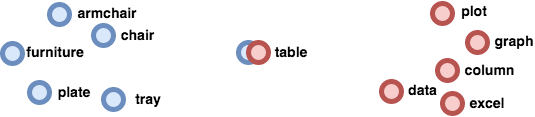
\includegraphics[width=1.0\textwidth]{figures/table-ambigous}
\end{center}	
\end{frame}

\begin{frame}{Word vs sense embeddings}

\begin{center}
	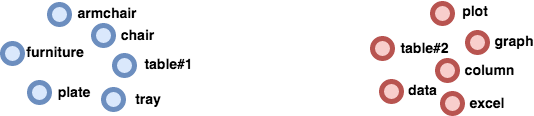
\includegraphics[width=1.0\textwidth]{figures/table-unambigous}
\end{center}	
\end{frame}


\begin{frame}[fragile]
\frametitle{Related work}
\begin{center}
 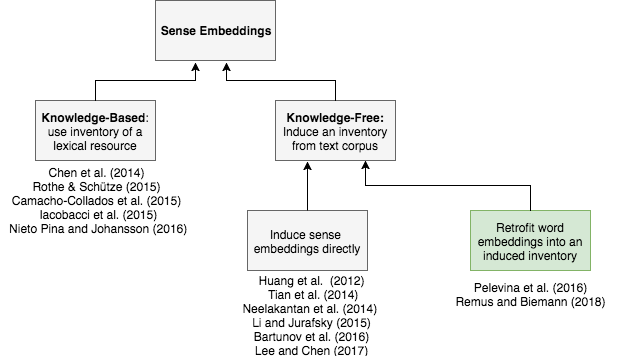
\includegraphics[height=0.56\textwidth]{figures/GWC-1}
 \end{center}
\end{frame}


\begin{frame}
\frametitle{Related work: knowledge-based}
\begin{itemize}
	\item \textbf{AutoExtend}~\cite{rothe-schutze:2015:ACL-IJCNLP}
\end{itemize}
\begin{center}
 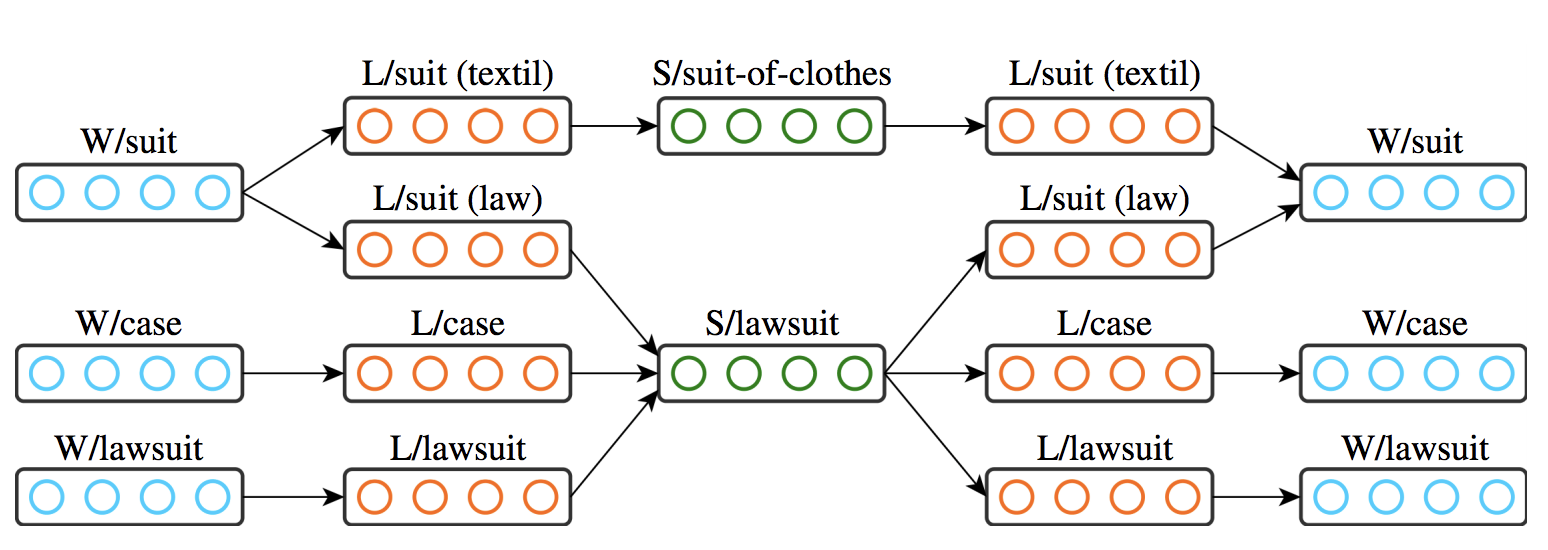
\includegraphics[width=1.0\textwidth]{figures/autoextend}
 \end{center}

{\footnotesize
 * image is reproduced from the original paper
}

\end{frame}

\begin{frame}{Related work: knowledge-free}

\begin{itemize}
\item \textbf{Adagram}~\cite{bartunov2016breaking}
\item Multiple vector representations $\theta$ for each word:

\pause
%$$p(Y|X,\theta)$$

 $$p(Y,\textcolor{Cerulean}{Z},\mathbf{\beta}|X,\alert{\alpha},\theta) = \prod_{w=1}^{V} \prod_{k=1}^{\infty} p(\beta_{wk}|\alert{\alpha}) \prod_{i=1}^N [p(\textcolor{Cerulean}{z_i}|x_i,\mathbf{\beta}) \prod_{j=1}^C p(y_{ij}|\textcolor{Cerulean}{z_i},x_i,\theta)],$$ 
\begin{itemize}
 
\item $\textcolor{Cerulean}{z_i}$ -- a hidden variable: a sense index of word $x_i$ in context $C$; 
\item $\alert{\alpha}$ -- a meta-parameter controlling number of senses.
%\item $p(\beta_{wk}|\alpha)$ -- probability of the $k$-th sense of the word $w$;
%\item $p(z_i|x_i,\mathbf{\beta})$ -- probability of observing word $x_i$ in the sense $z_i$;
%\item $\prod_{j=1}^C p(y_{ij}|z_i,x_i,\theta)$ -- probability of the context $C$.
\end{itemize}

\pause 
\item \alert{\textbf{See also}}: [Neelakantan et al., 2014] and [Li and Jurafsky, 2015]

\end{itemize}
	
\end{frame}


\begin{frame}{Related work: word sense induction}

\begin{itemize}
	\item Word sense induction (WSI) based on \alert{\textbf{graph clustering}}:  
	\begin{itemize}
	\item $ $ [Lin, 1998]
	\item $ $ [Pantel and Lin, 2002]
	\item $ $ [Widdows and Dorow, 2002]
	\item $ $ \textbf{Chinese Whispers [Biemann, 2006]}
	\item $ $ [Hope and Keller, 2013]
	\end{itemize}
	
	%\item ...we extend this line of work.
\end{itemize}
	

\end{frame}



\begin{frame}[fragile]
\frametitle{Related work: Chinese Whispers\#1}
\begin{center}
 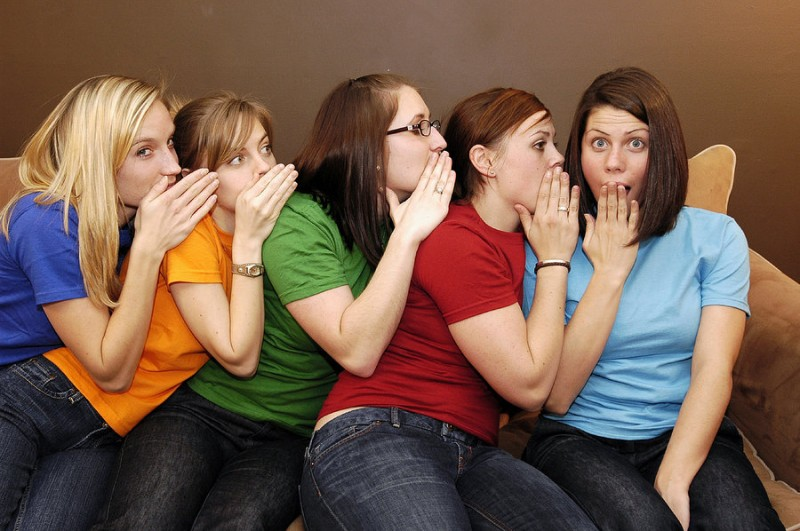
\includegraphics[height=0.5\textwidth]{figures/cw}
 
  {\tiny * source of the image: \url{http://ic.pics.livejournal.com/blagin_anton/33716210/2701748/2701748_800.jpg}}
 \end{center}
\end{frame}



\begin{frame}[fragile]
\frametitle{Related work: Chinese Whispers\#2}
\begin{center}
 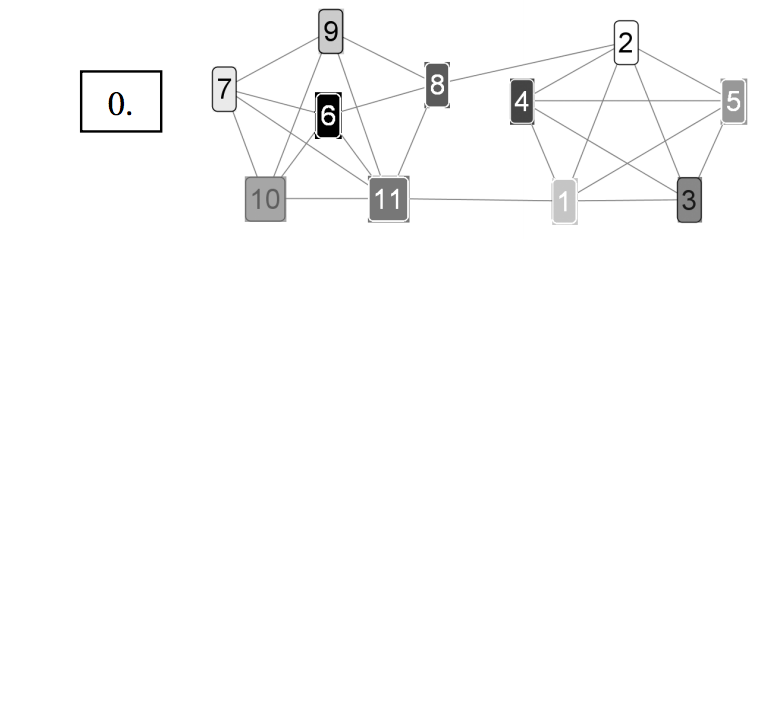
\includegraphics[height=0.59\textwidth]{figures/cw2-1}
 
  %{\tiny * source of the image: [Biemann, 2006]}
 \end{center}
\end{frame}


\begin{frame}[fragile]
\frametitle{Related work: Chinese Whispers\#2}
\begin{center}
 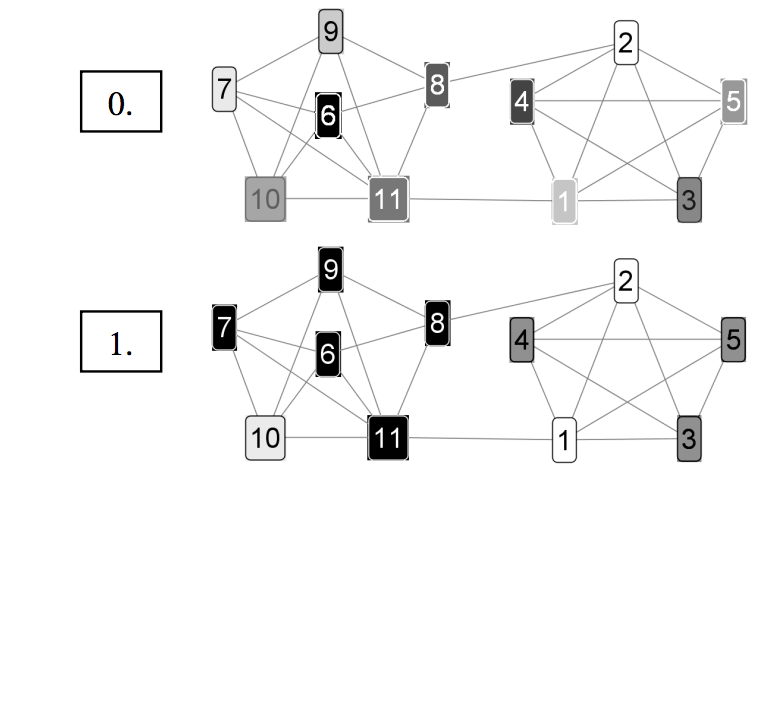
\includegraphics[height=0.59\textwidth]{figures/cw2-2}
 
  %{\tiny * source of the image: [Biemann, 2006]}
 \end{center}
\end{frame}

\begin{frame}[fragile]
\frametitle{Related work: Chinese Whispers\#2}
\begin{center}
 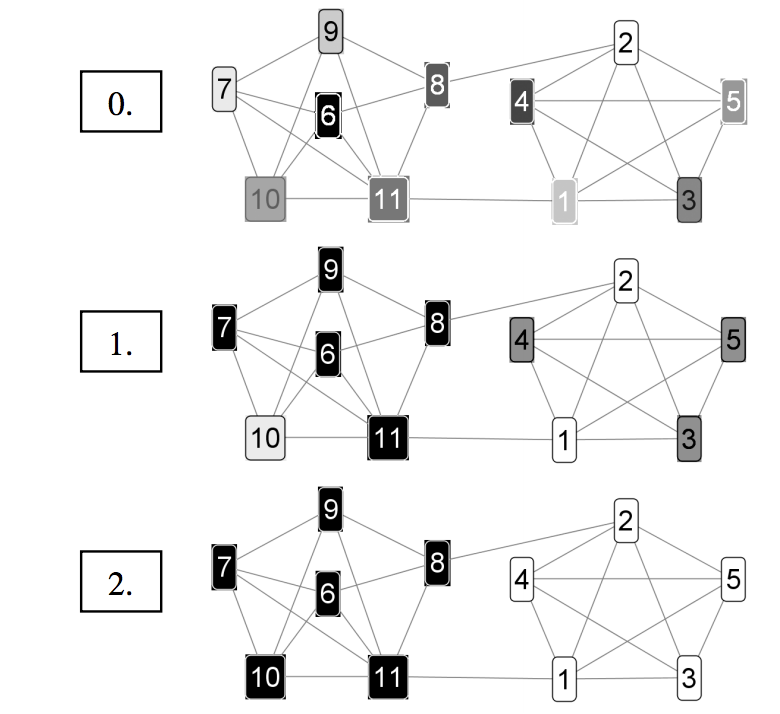
\includegraphics[height=0.59\textwidth]{figures/cw2}
 
  %{\tiny * source of the image: [Biemann, 2006]}
 \end{center}
\end{frame}



\begin{frame}{Sense embeddings using retrofitting}
	
	%\begin{itemize} 
	 {\footnotesize \textbf{RepL4NLP@ACL'16} \cite{pelevina-EtAl:2016:RepL4NLP}, \textbf{LREC'18} \cite{remus:2018}}
	%\end{itemize}
	
	\begin{block}{Prior methods:}
		\vspace{0.25cm}

	\begin{itemize}	
	\item Induce inventory by \alert{clustering of word instances} %(Li and Jurafsky, 2015)
	\item Use \alert{existing} sense inventories %(Rothe and Sch\"{u}tze, 2015)	
	\end{itemize}
\end{block}


	\begin{block}{Our method:}
		\vspace{0.25cm}

	\begin{itemize}	
	\item \textbf{Input:} word embeddings
	\item \textbf{Output:} word sense embeddings
	\item \textbf{Word sense induction} by \alert{clustering of word ego-networks}
	%\item \textbf{Word sense disambiguation} based on the induced sense representations

	\end{itemize}
\end{block}


\end{frame}

\begin{frame}{Sense embeddings using retrofitting}
\begin{itemize}
\item From word embeddings to sense embeddings
\end{itemize}
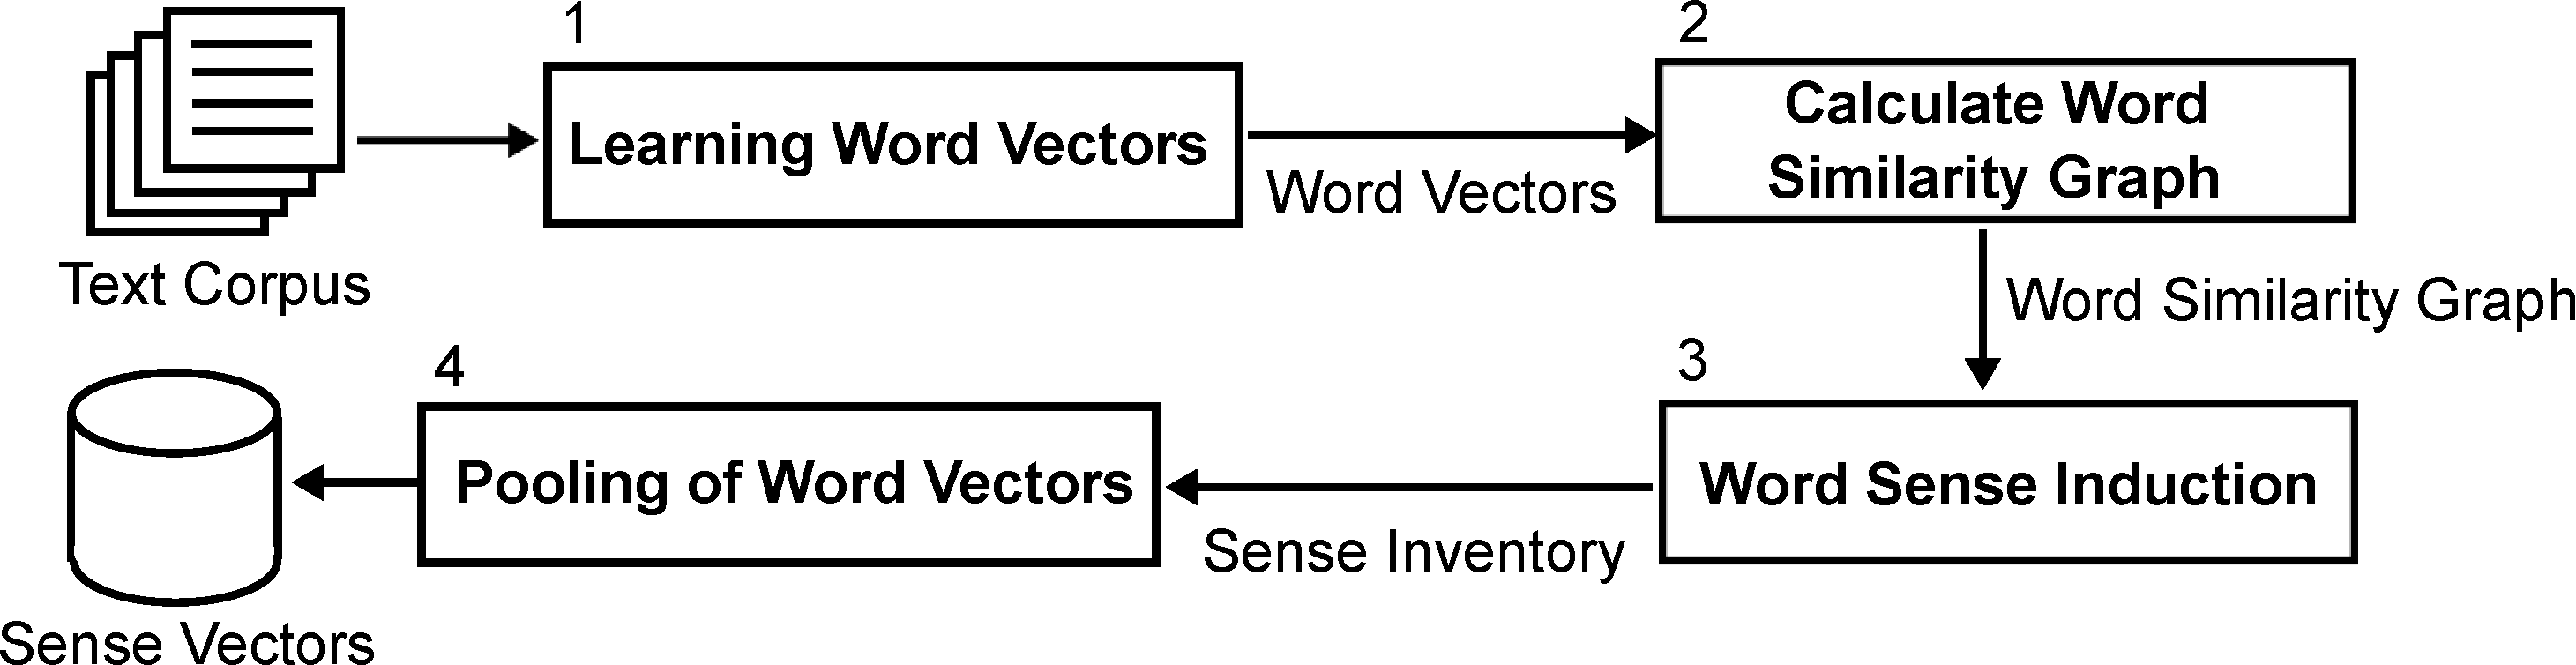
\includegraphics[width=\textwidth]{figures/pipeline-sensegram}
%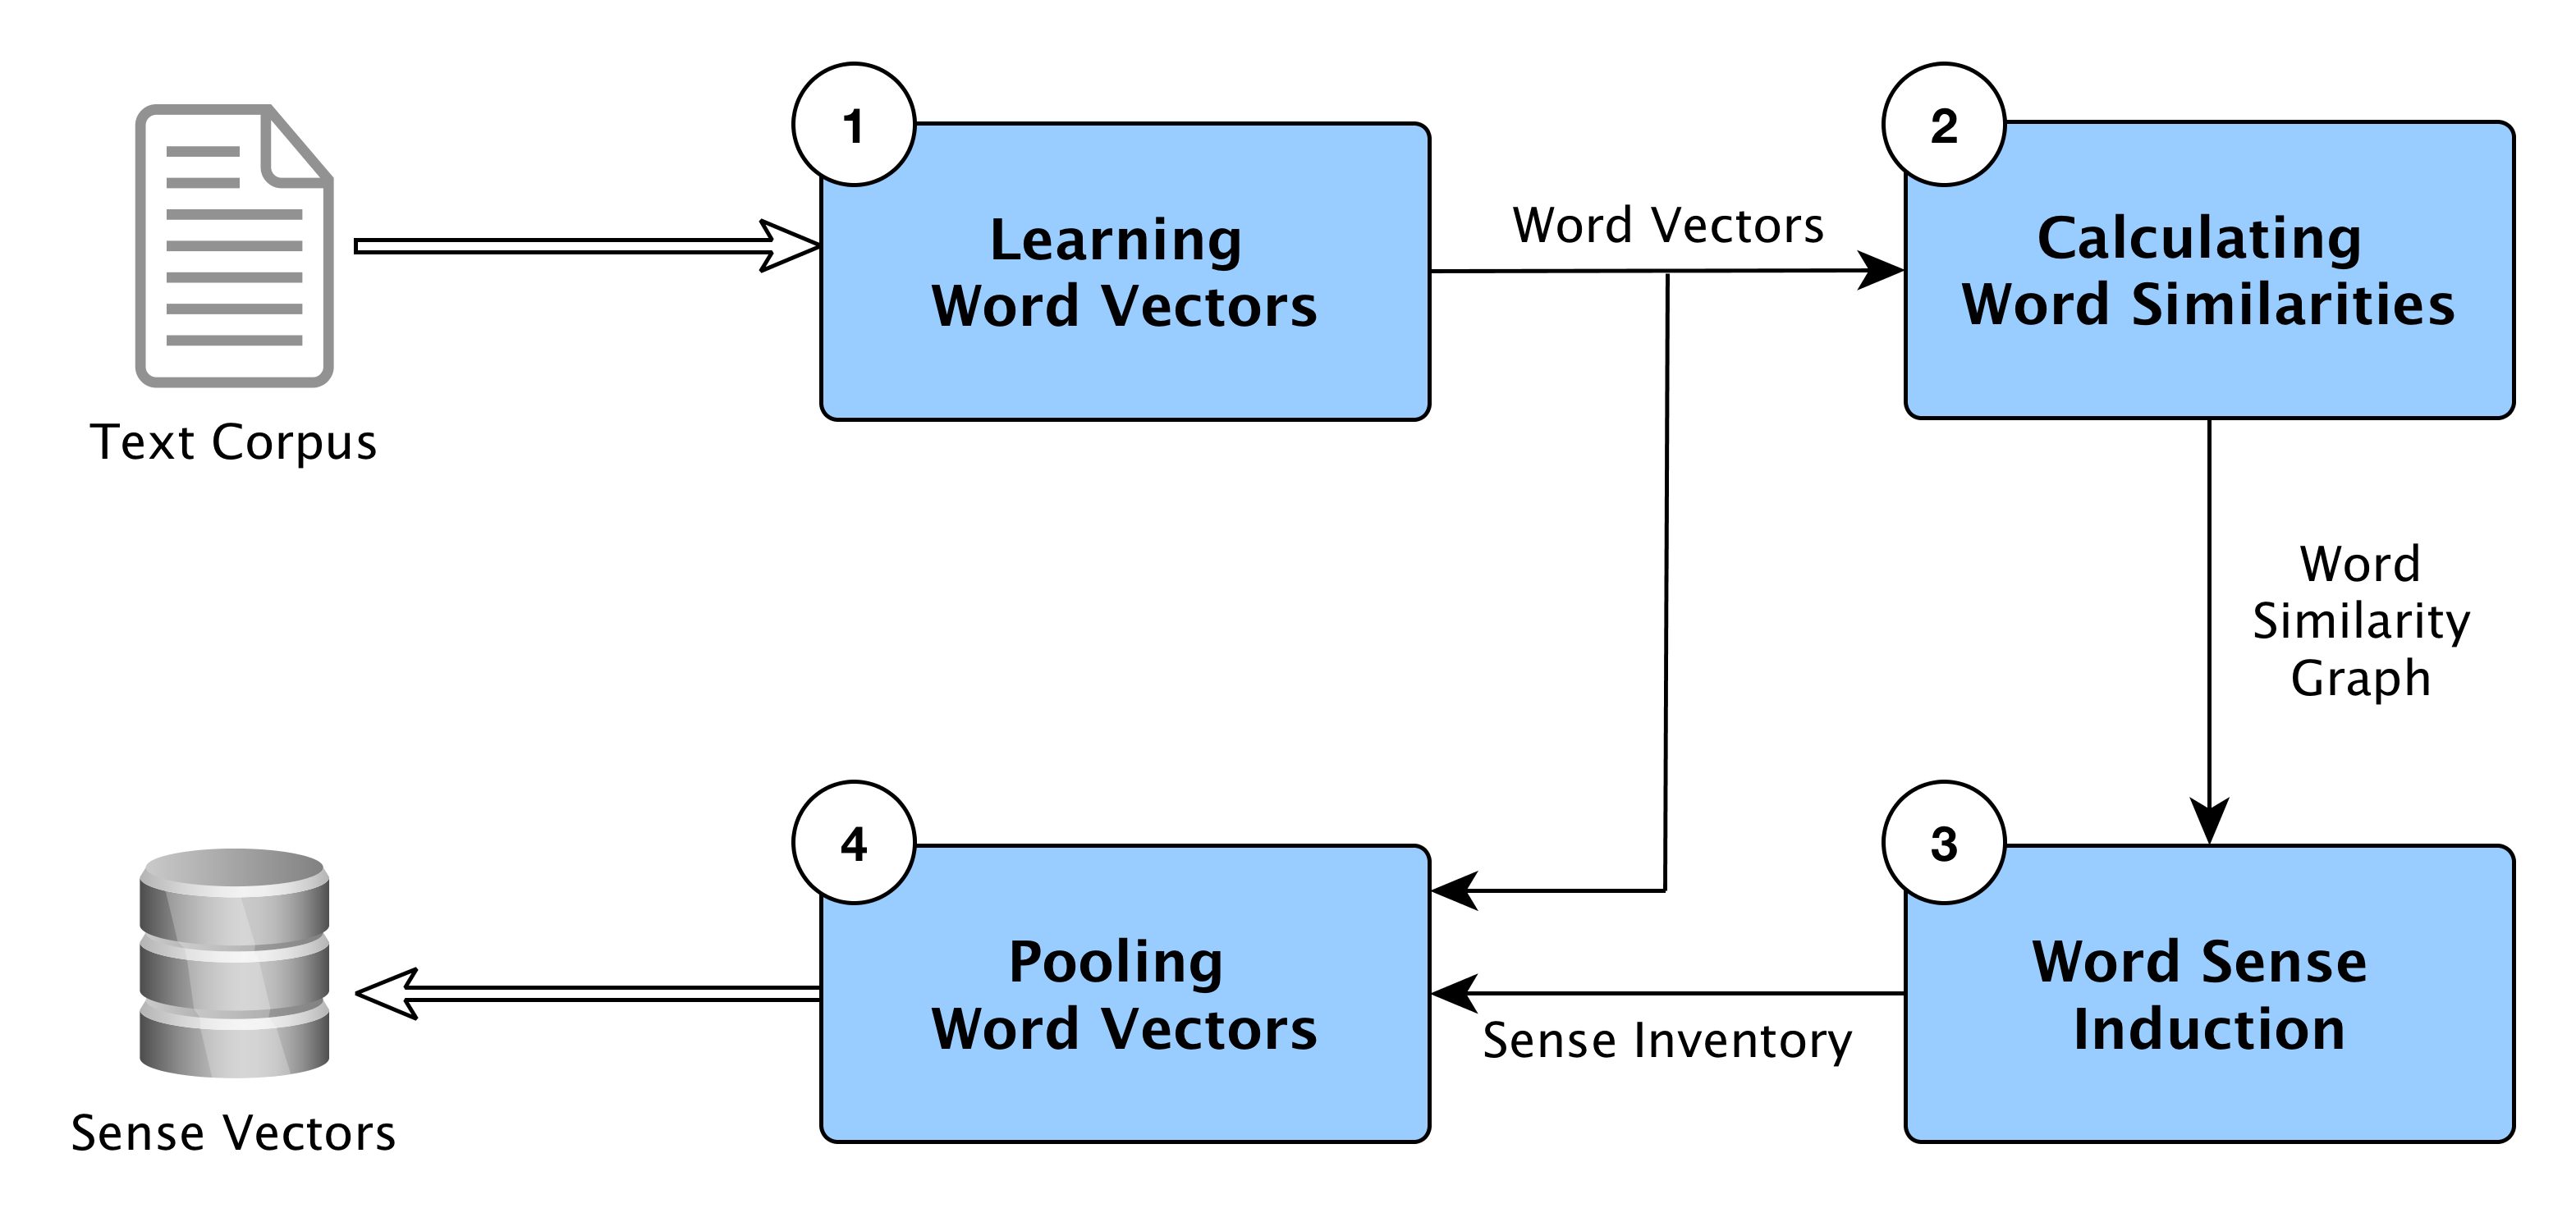
\includegraphics[width=\textwidth]{pipeline}

\end{frame}



\begin{frame}{Sense embeddings using retrofitting}

\begin{itemize}
\item Word sense induction using  ego-network clustering
\end{itemize} 
	
\centering
\begin{figure}
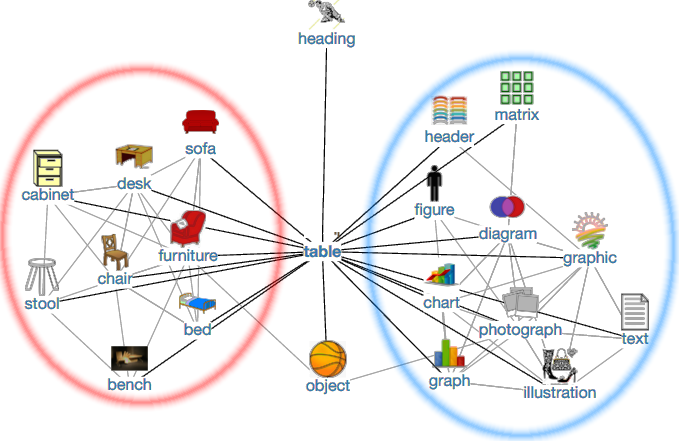
\includegraphics[width=0.75\textwidth]{figures/table}
\end{figure}

\end{frame}


\begin{frame}{Sense embeddings using retrofitting}

\begin{itemize}
	\item Neighbours of Word and Sense Vectors
\end{itemize}


%\begin{table}
%
%\footnotesize
%\centering

\begin{tabular}{l|p{9cm}}
\bf Vector & \bf {Nearest Neighbors} \\ \toprule
 table & $ $ \alert{tray}, \textcolor{Cerulean}{bottom}, \textcolor{Cerulean}{diagram}, \alert{bucket}, \textcolor{Cerulean}{brackets}, \textcolor{Cerulean}{stack}, \alert{basket}, \textcolor{Cerulean}{list}, \textcolor{Cerulean}{parenthesis}, \alert{cup}, \alert{saucer}, \alert{pile}, \alert{playfield}, \textcolor{Cerulean}{bracket}, \alert{pot}, \textcolor{Cerulean}{drop-down}, \alert{cue}, \alert{plate} \\ \midrule
 \pause
  \textcolor{Cerulean}{table\#0} & $ $ \textcolor{Cerulean}{leftmost\#0},  \textcolor{Cerulean}{column\#1},  \textcolor{Cerulean}{tableau\#1},  \textcolor{Cerulean}{indent\#1},  \textcolor{Cerulean}{bracket\#3},  \textcolor{Cerulean}{pointer\#0},  \textcolor{Cerulean}{footer\#1}, \textcolor{Cerulean}{cursor\#1}, \textcolor{Cerulean}{diagram\#0}, \textcolor{Cerulean}{grid\#0} \\ \midrule
   \alert{table\#1} & $ $ \alert{pile\#1,  stool\#1,  tray\#0,  basket\#0,  bowl\#1,  bucket\#0,  box\#0,  cage\#0,  saucer\#3,      mirror\#1,  pan\#1,  lid\#0}  \\ 
\end{tabular}
	

\end{frame}




\begin{frame}{Sense embeddings using retrofitting}
	
	\begin{block}{Word Sense Disambiguation}
	
	\begin{enumerate} 
	\item \textbf{\alert{Context extraction}}: use context words around the target word
	\item \textbf{\alert{Context filtering}}: based on context word's relevance for disambiguation
	
	\item \textbf{\alert{Sense choice in context}}: maximise similarity between a context vector and a sense vector
	
	\end{enumerate}
	\end{block}

\end{frame}


\begin{frame}{Sense embeddings using retrofitting}
\vspace{-3em}
\begin{center}
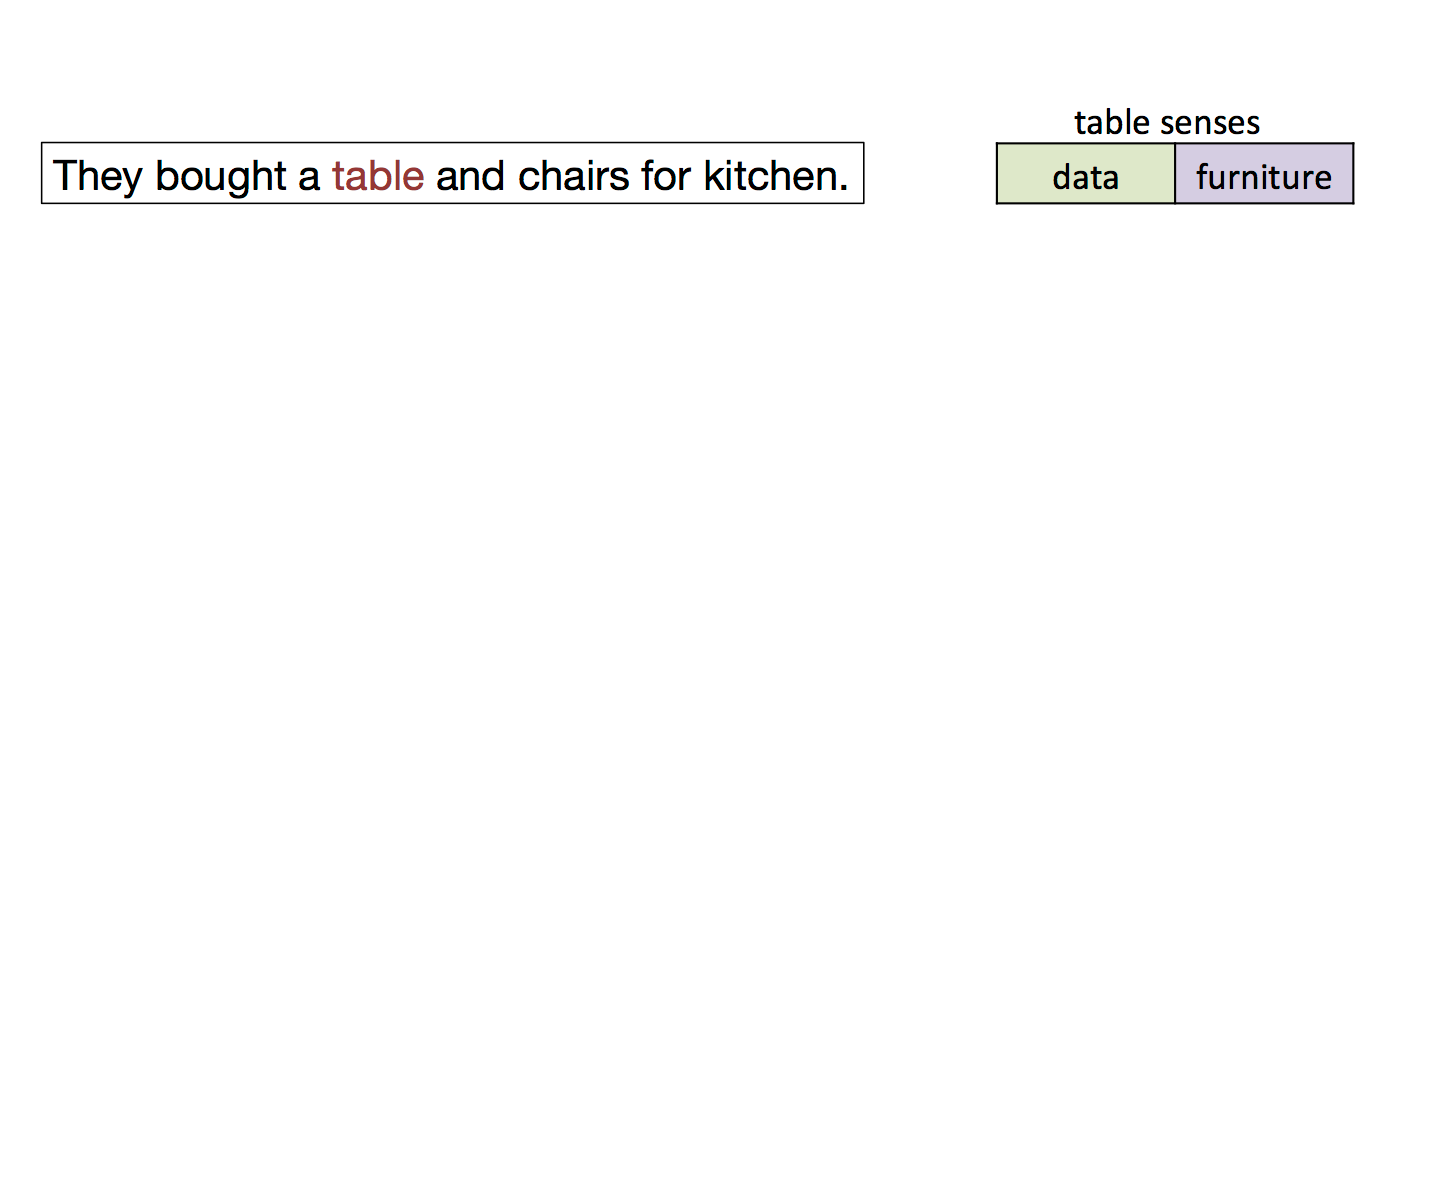
\includegraphics[width=0.82\textwidth]{figures/wsd-1}
\end{center}	
\end{frame}



\begin{frame}{Sense embeddings using retrofitting}
\vspace{-3em}
\begin{center}
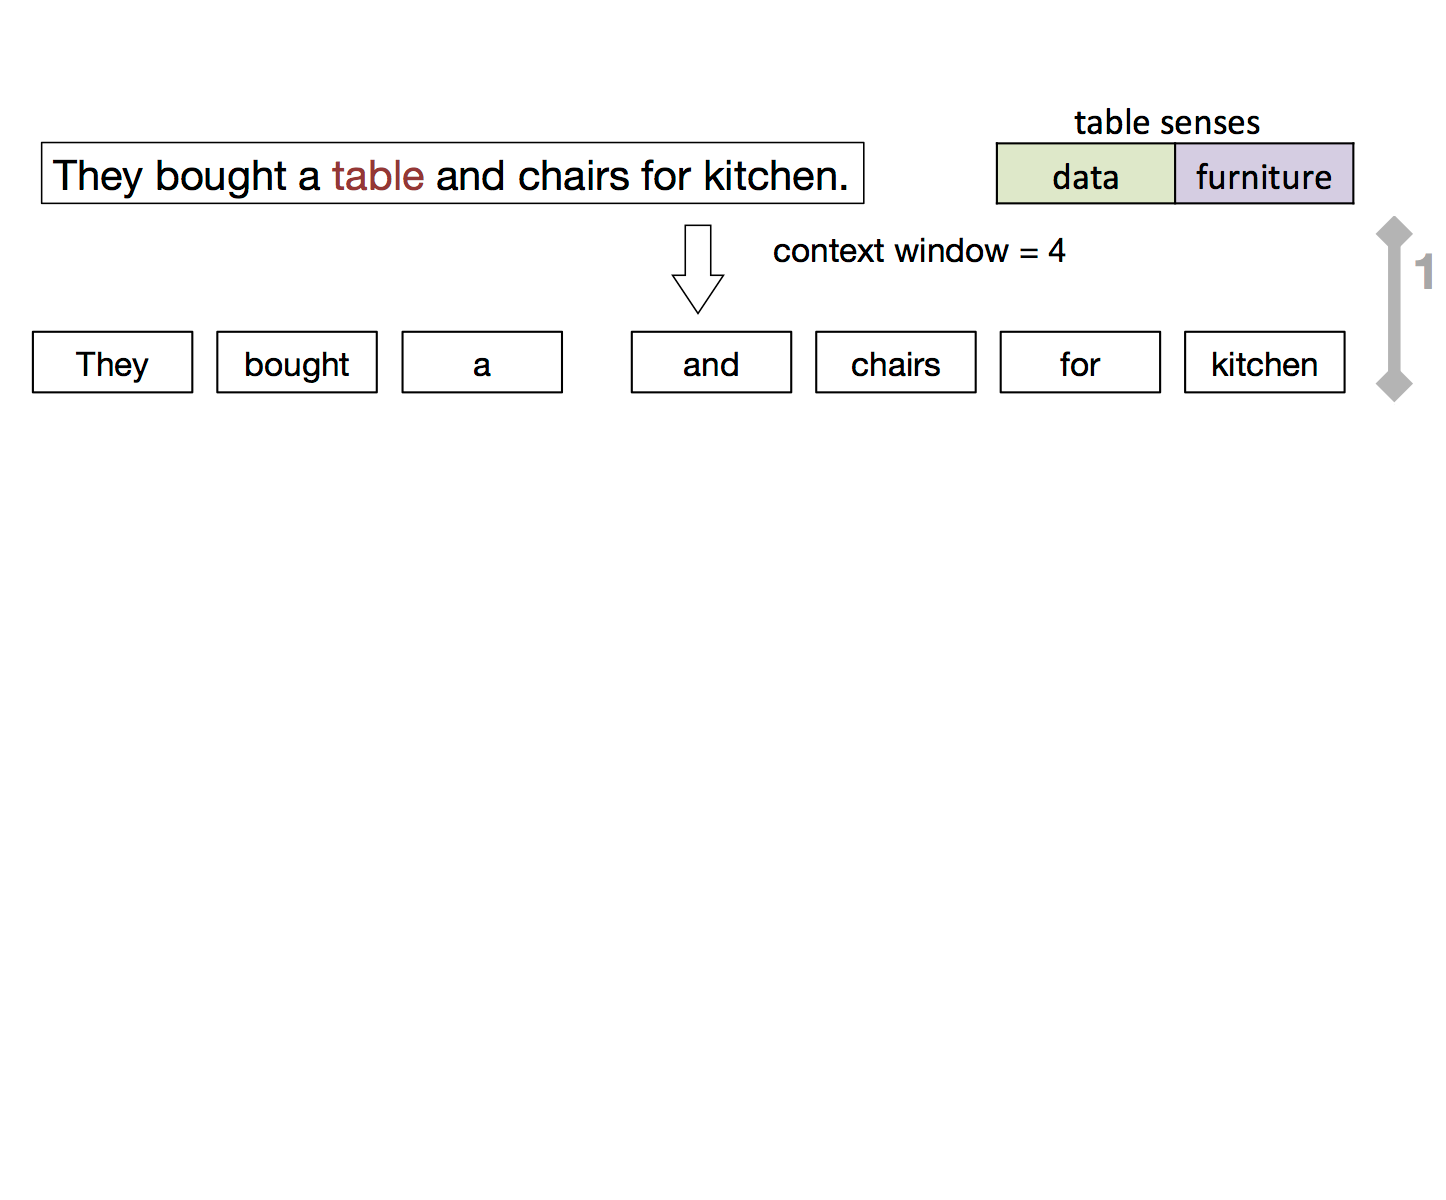
\includegraphics[width=0.82\textwidth]{figures/wsd-2}
\end{center}	
\end{frame}



\begin{frame}{Sense embeddings using retrofitting}
\vspace{-3em}
\begin{center}
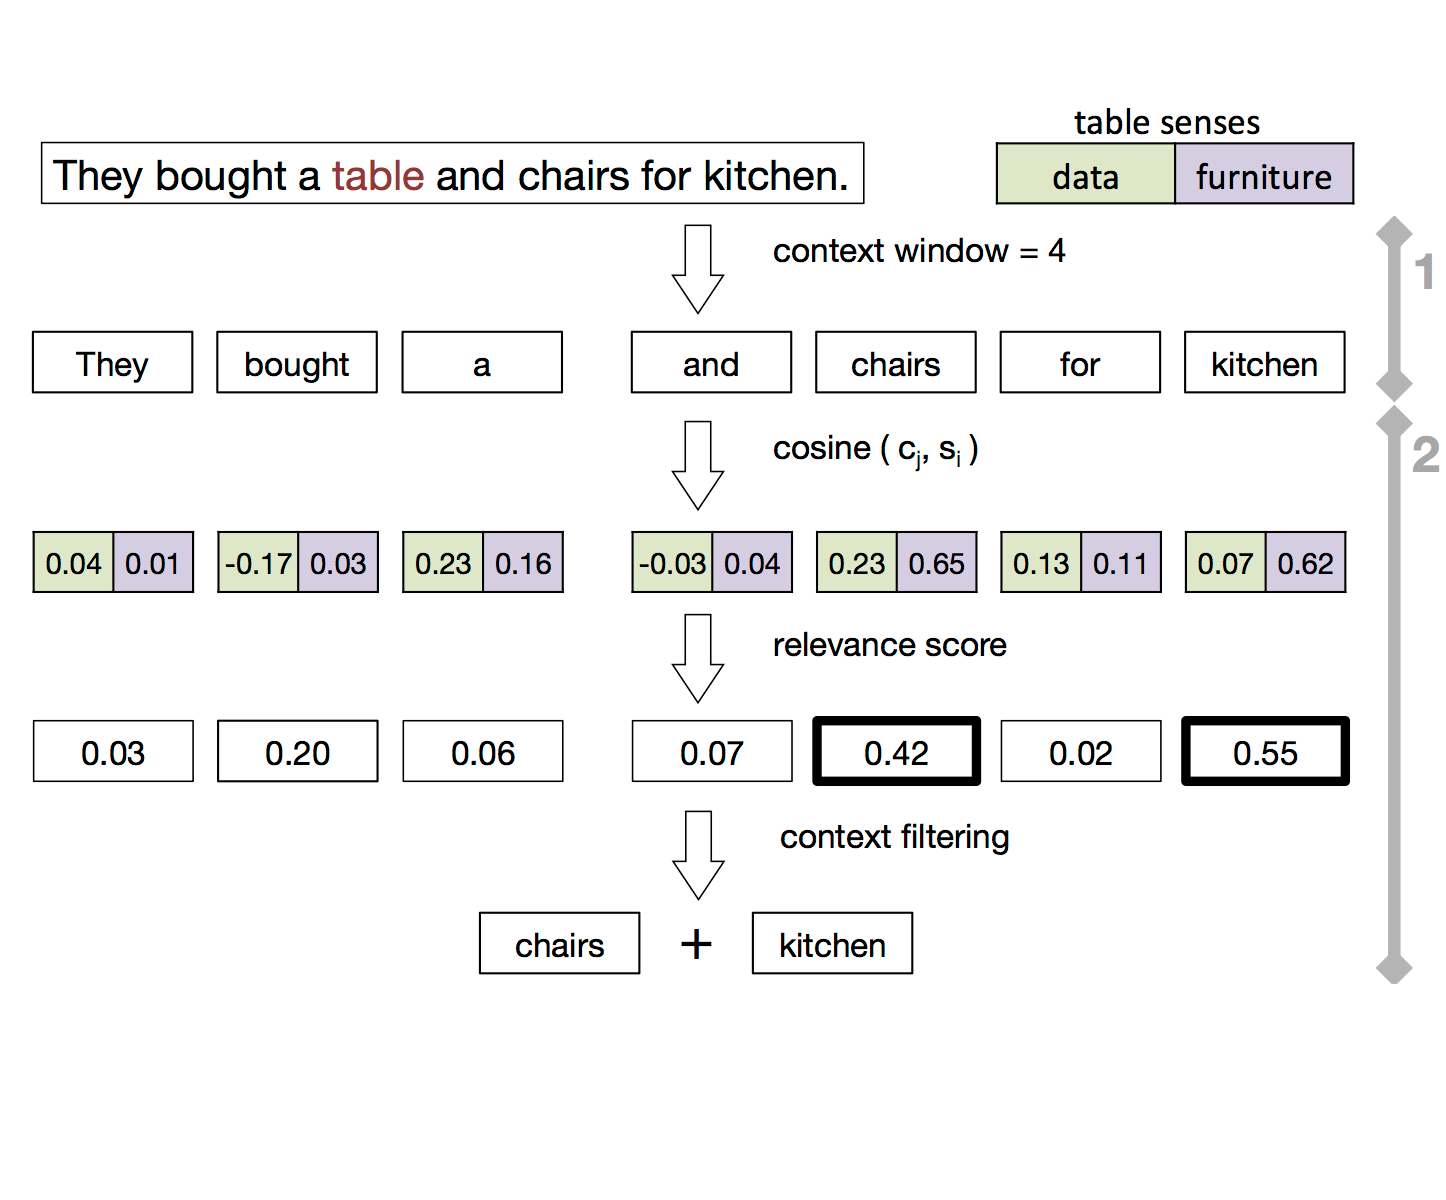
\includegraphics[width=0.82\textwidth]{figures/wsd-3}
\end{center}	
\end{frame}



	
\begin{frame}{Sense embeddings using retrofitting}
%\begin{itemize}
%	\item An example of word sense disambiguation
%\end{itemize}
\vspace{-3em}
	\begin{center}
		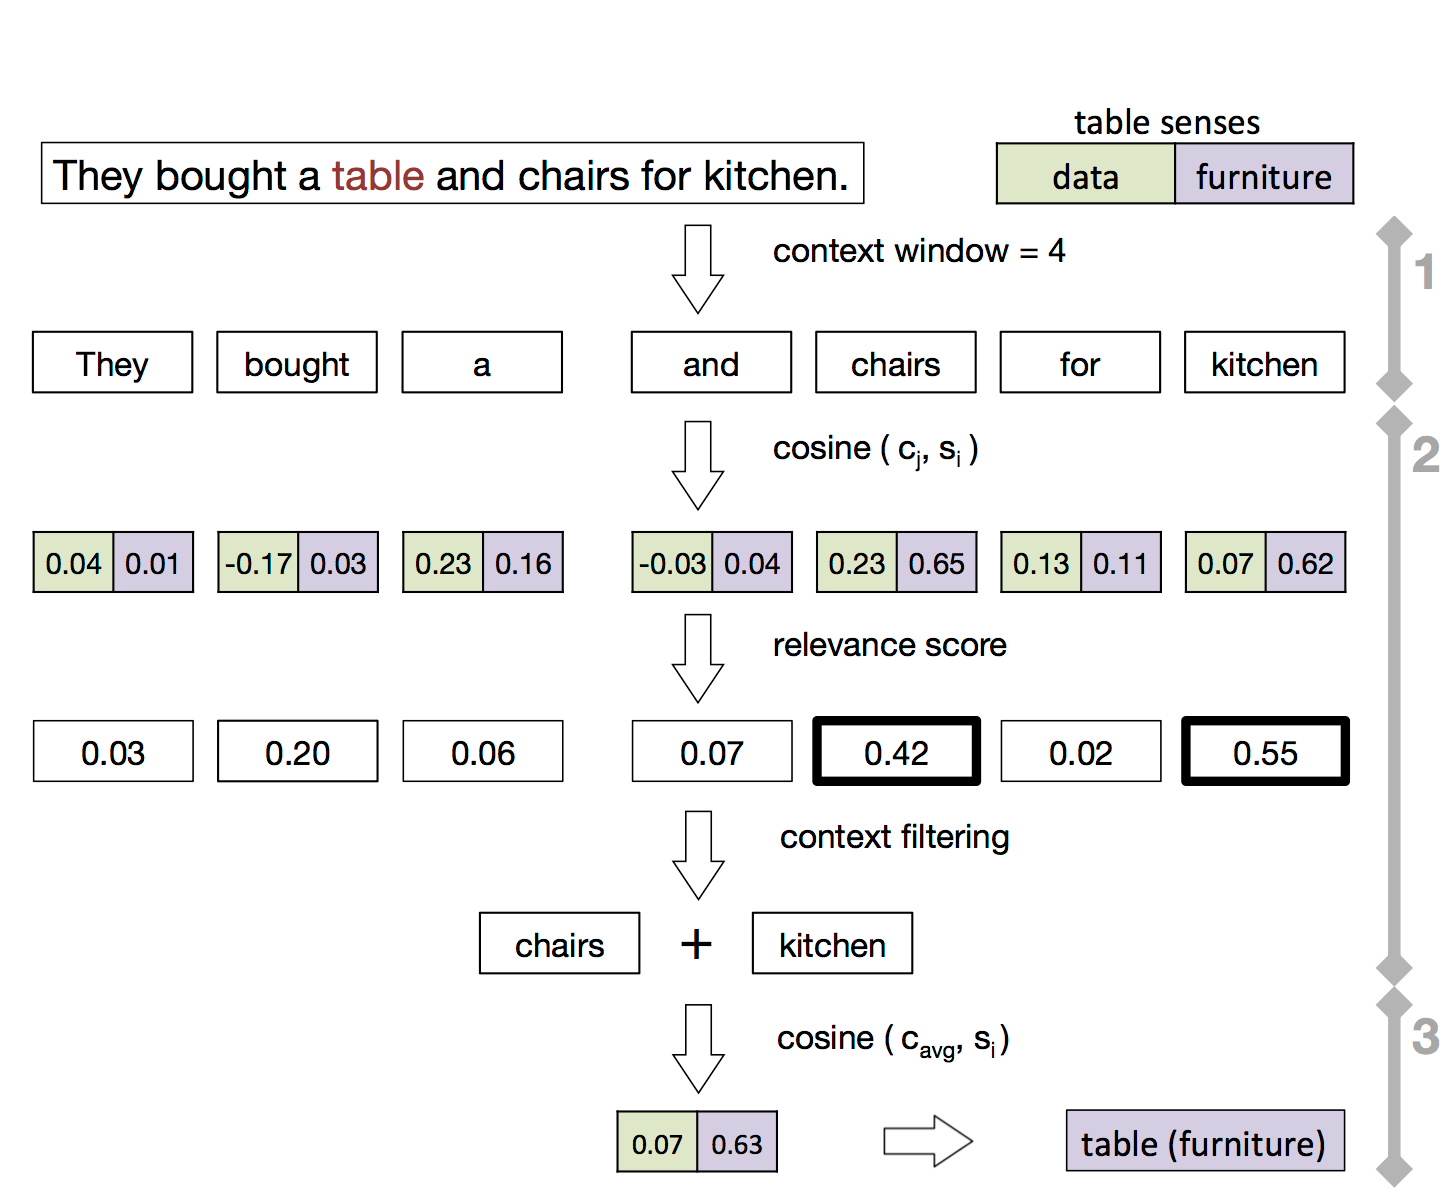
\includegraphics[width=0.82\textwidth]{figures/wsd}
	\end{center}
	
\end{frame}






\begin{frame}{Sense embeddings using retrofitting}

\alert{\textbf{Unsupervised WSD}} SemEval'13, \textbf{ReprL4NLP}~\cite{pelevina-EtAl:2016:RepL4NLP}:
\begin{itemize}
	\item comparable to SOTA, incl. Adagram sense embeddings.
\end{itemize} 

\pause
\vspace{2em}
\alert{\textbf{Semantic relatedness}}, \textbf{LREC'2018}~\cite{remus:2018}:
\vspace{2em}
\begin{table}
    \tiny
 	
 	\def\arraystretch{1.2}% 
 	\setlength{\arraycolsep}{3pt}
 	
 	$$
 	\begin{array}{rll|ll|ll|ll|ll|ll|ll}
 	  & \rotatebox{80}{\textsc{autoextend}\hspace{-10em}} 
 	  & \rotatebox{80}{\textsc{adagram}\hspace{-10em}} 
 	  & ~\rotatebox{80}{\textsc{SGNS}\hspace{-10em}} 
 	  & \rotatebox{80}{\textsc{.}\hspace{-10em}} 
 	  & \rotatebox{80}{\textsc{glove}\hspace{-10em}} 
 	  & \rotatebox{80}{\textsc{.}\hspace{-10em}} 
 	  & \rotatebox{80}{\textsc{sympat}\hspace{-10em}} 
 	  & \rotatebox{80}{\textsc{.}\hspace{-10em}} 
 	  & \rotatebox{80}{\textsc{LSAbow}\hspace{-10em}} 
 	  & \rotatebox{80}{\textsc{.}\hspace{-10em}}
 	  & \rotatebox{80}{\textsc{LSAhal}\hspace{-10em}}
	  & \rotatebox{80}{\textsc{.}\hspace{-10em}}
	  & ~~\rotatebox{80}{\textsc{paragramSL}\hspace{-10em}} 
 	  & \rotatebox{80}{\textsc{.}\hspace{-10em}}  
 	  \\
   	 \textsc{SimLex999}  & 0.45 & 0.29 ~~&~ 0.44 &  & 0.37 &  & 0.54 &  & 0.30 &  & 0.27 & & ~ {0.68} &  \\
   	 \textsc{MEN} & 0.72 & 0.67 &~   0.77 &  & 0.73 &  & 0.53 &  & 0.67 &  & 0.71 &  &~ 0.77 &  \\
   	 \textsc{SimVerb} & 0.43 & 0.27 &~   0.36 &  & 0.23 &  & 0.37 &  & 0.15 &  & 0.19 &  &~ 0.53 &  \\
   	 \textsc{WordSim353} & 0.58 & 0.61 &~   {0.70} &  & 0.61 &  & 0.47 & & {0.67} &  & 0.59 & &~ 0.72 & \\ 

   	 \textsc{SimLex999-N}  & 0.44 & 0.33 ~~&~ 0.45 &  & 0.39 &  & 0.48 &  & 0.32 & & 0.34 & & {0.68} & \\
   	 \textsc{MEN-N} 		 & 0.72 & 0.68 &~   0.77 & \_\_\_\_ & 0.76 & \_\_\_\_ & 0.57 & \_\_\_\_ & 0.71 & \_\_\_\_ & 0.73 & \_\_\_\_ &~ 0.78 & \_\_\_\_ \\
 	\end{array}
 	$$
 
 \end{table}


\end{frame}



\begin{frame}{Sense embeddings using retrofitting}

\alert{\textbf{Unsupervised WSD}} SemEval'13, \textbf{ReprL4NLP}~\cite{pelevina-EtAl:2016:RepL4NLP}:
\begin{itemize}
	\item comparable to SOTA, incl. sense embeddings.
\end{itemize} 

\vspace{2em}

\alert{\textbf{Semantic relatedness}}, \textbf{LREC'2018}~\cite{remus:2018}:
\vspace{2em}
\begin{table}
    \tiny
 	
 	\def\arraystretch{1.2}% 
 	\setlength{\arraycolsep}{3pt}
 	
 	$$
 	\begin{array}{rll|ll|ll|ll|ll|ll|ll}
 	  & \rotatebox{80}{\textsc{autoextend}\hspace{-10em}} 
 	  & \rotatebox{80}{\textsc{adagram}\hspace{-10em}} 
 	  & ~\rotatebox{80}{\textsc{SGNS}\hspace{-10em}} 
 	  & \rotatebox{80}{\textsc{SGNS\alert{+senses}}\hspace{-10em}} 
 	  & \rotatebox{80}{\textsc{glove}\hspace{-10em}} 
 	  & \rotatebox{80}{\textsc{glove\alert{+senses}}\hspace{-10em}} 
 	  & \rotatebox{80}{\textsc{sympat}\hspace{-10em}} 
 	  & \rotatebox{80}{\textsc{sympat\alert{+senses}}\hspace{-10em}} 
 	  & \rotatebox{80}{\textsc{LSAbow}\hspace{-10em}} 
 	  & \rotatebox{80}{\textsc{LSAbow\alert{+senses}}\hspace{-10em}}
 	  & \rotatebox{80}{\textsc{LSAhal}\hspace{-10em}}
	  & \rotatebox{80}{\textsc{LSAhal\alert{+senses}}\hspace{-10em}}
	  & ~~\rotatebox{80}{\textsc{paragramSL}\hspace{-10em}} 
 	  & \rotatebox{80}{\textsc{paragramSL\alert{+senses}}\hspace{-10em}}  
 	  \\
   	 \textsc{SimLex999}  & 0.45 & 0.29 ~~&~ 0.44 & \mathbf{0.46} & 0.37 & \bf0.41 & 0.54 & \mathbf{0.55} & 0.30 & \bf0.39 & 0.27 & \bf0.38 ~& \mathbf{0.68} & {0.64} \\
   	 \textsc{MEN} 		 & 0.72 & 0.67 &~   0.77 & \mathbf{0.78} & 0.73 & \bf0.77 & 0.53 & \bf0.68 & 0.67 & \bf0.70 & 0.71 & \bf0.74 &~ 0.77 & \bf0.80  \\
   	 \textsc{SimVerb} 	 & 0.43 & 0.27 &~   0.36 & \bf0.39 & 0.23 & \bf0.30 & 0.37 & \bf0.45 & 0.15 & \bf0.22 & 0.19 & \bf0.28 & 0.53 & 0.53 \\
   	 \textsc{WordSim353} & 0.58 & 0.61 &~   \mathbf{0.70} & 0.69 & 0.61 & \bf0.65 & 0.47 & \bf0.62 & \mathbf{0.67} & 0.66 & 0.59 & \bf0.63 &~ 0.72 & \mathbf{0.73} \\ 

   	 \textsc{SimLex999-N}  & 0.44 & 0.33 ~~&~ 0.45 & \bf0.50 & 0.39 & \bf0.47 & 0.48 & \bf0.55 & 0.32 & \bf0.46 & 0.34 & \bf 0.44 & \mathbf{0.68} & {0.66} \\
   	 \textsc{MEN-N} 		 & 0.72 & 0.68 &~   0.77 & \mathbf{0.79} & 0.76 & \bf0.80 & 0.57 & \bf0.74 & 0.71 & \mathbf{0.73} & 0.73 & \bf0.76 &~ 0.78 & \bf 0.81 \\
 	\end{array}
 	$$
 
 \end{table}
%\vspace{-1em}
%\begin{itemize}
%
%\item Sense-aware similarities are marked with \alert{\textsc{+SENSES}}.
%\item These results are using a sense inventory based on \textbf{sparse dependency features} (JoBimText).
%
%\end{itemize}

\end{frame}



\begin{frame}{Sense embeddings using retrofitting}
\vspace{-1em}
\begin{columns}
\begin{column}{0.55\textwidth}
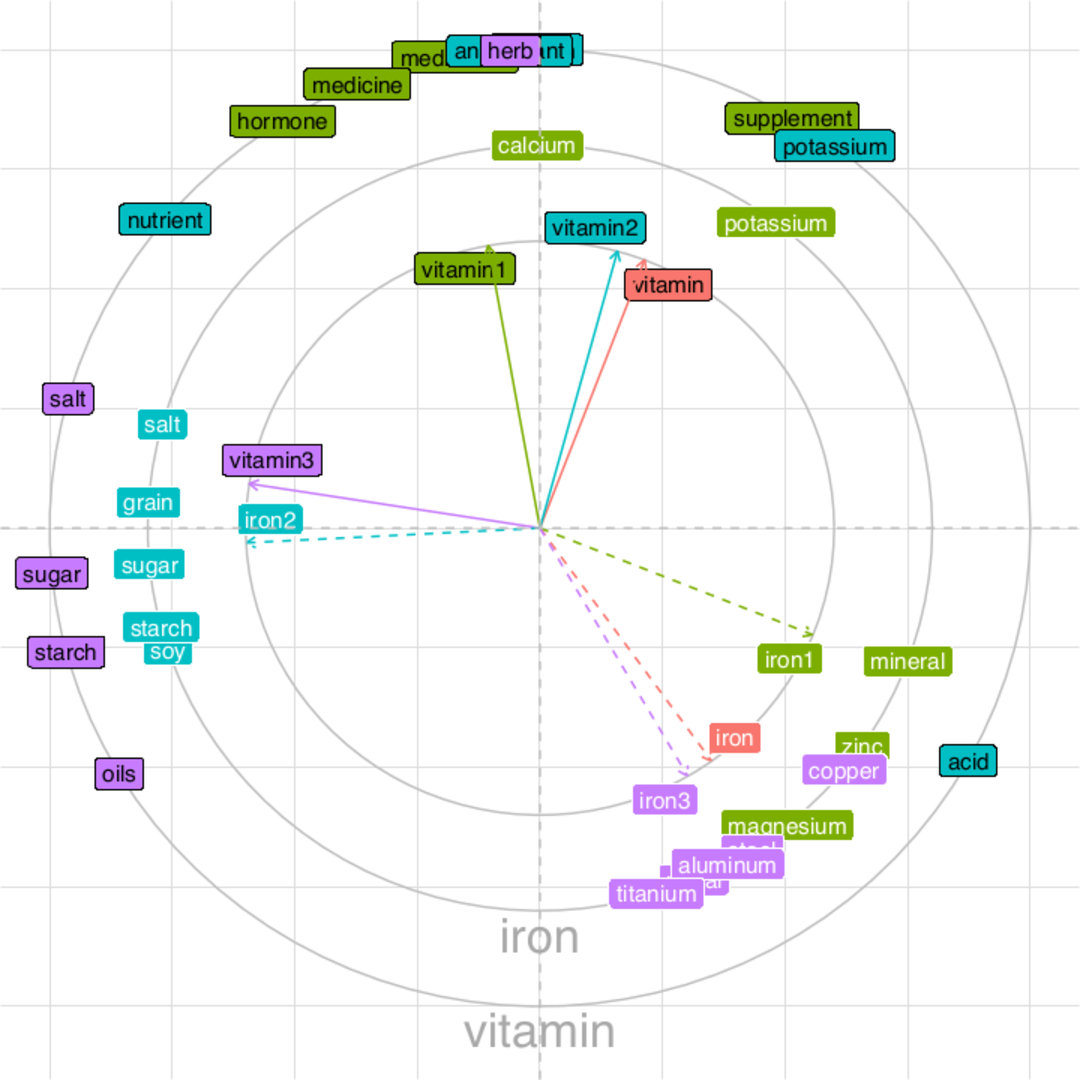
\includegraphics[height=0.68\textheight]{figures/bullseye}
\end{column}

\begin{column}{.45\textwidth}
{ \footnotesize

\begin{itemize}

\item Word and sense embeddings of words \textbf{iron} and  \textbf{vitamin}.

\end{itemize}

\textbf{LREC'18}~\cite{remus:2018}

}
\end{column}
\end{columns}

\end{frame}

%%%%%%%%%%%%%%%%%%%%%%%%% 
